
%(BEGIN_QUESTION)
% Copyright 2010, Tony R. Kuphaldt, released under the Creative Commons Attribution License (v 1.0)
% This means you may do almost anything with this work of mine, so long as you give me proper credit

This control system tries to maintain the water level at a constant value inside the boiler's steam drum by adding ``feed'' water to the bottom drum as steam evaporates off the top drum:

$$\includegraphics[width=15.5cm]{i04430x01.eps}$$

Assuming both the level transmitter (LT) and I/P converter (LY) are direct-acting (i.e. increasing input = increasing output), and that the level controller is perfectly tuned, answer the following questions:

\begin{itemize}
\item{} Determine the proper control action of the LIC (either {\it direct} or {\it reverse}).
\vskip 10pt
\item{} Calculate the necessary $C_v$ rating of the feedwater valve, assuming a maximum desired flowrate of 58 gallons per minute with a pump pressure of 380 PSIG and a boiler pressure of 350 PSIG.
\vskip 10pt
\item{} Determine what will happen to the boiler water level ({\it increase}, {\it decrease}, or {\it remain essentially constant}) if an operator slightly opens the manual bypass valve when the boiler is outputting full steam flow.  Normally, this manual bypass valve is in the fully closed position.
\vskip 10pt
\item{} Determine what will happen to the controller output signal ({\it increase}, {\it decrease}, or {\it remain essentially constant}) if an operator slightly opens the manual bypass valve when the boiler is outputting full steam flow.  Normally, this manual bypass valve is in the fully closed position.
\end{itemize}

%\item{} Determine what will happen to the boiler drum level ({\it increase}, {\it decrease}, or {\it remain essentially constant}) if an operator slightly opens the manual bypass valve when the boiler is in ``standby'' mode with zero steam usage.  Normally, this manual bypass valve is in the fully closed position.

\underbar{file i04430}
%(END_QUESTION)





%(BEGIN_ANSWER)

Each correct answer is worth 2.5 points:

\begin{itemize}
\item{} The LIC must be {\bf reverse} acting.
\vskip 10pt
\item{} $C_v$ = 10.589
\vskip 10pt
\item{} The boiler water level will {\bf remain essentially constant} if an operator slightly opens the manual bypass valve.
\vskip 10pt
\item{} The controller output signal will {\bf decrease} if an operator slightly opens the manual bypass valve.
\end{itemize}

%(END_ANSWER)





%(BEGIN_NOTES)

{\bf This question is intended for exams only and not worksheets!}.

%(END_NOTES)

